\documentclass[11pt]{charter}

% El títulos de la memoria, se usa en la carátula y se puede usar el cualquier lugar del documento con el comando \ttitle
\titulo{Equipo de monitoreo y trazabilidad de cadena de frío de medicamentos en tiempo real} 

% Nombre del posgrado, se usa en la carátula y se puede usar el cualquier lugar del documento con el comando \degreename
\posgrado{Carrera de Especialización en Sistemas Embebidos} 
%\posgrado{Carrera de Especialización en Internet de las Cosas} 
%\posgrado{Carrera de Especialización en Intelegencia Artificial}
%\posgrado{Maestría en Sistemas Embebidos} 
%\posgrado{Maestría en Internet de las cosas}

% Tu nombre, se puede usar el cualquier lugar del documento con el comando \authorname
\autor{Ing. Cristian Marcelo Funes} 

% El nombre del director y co-director, se puede usar el cualquier lugar del documento con el comando \supname y \cosupname y \pertesupname y \pertecosupname
\director{Ing. Ernesto Chediack}
\pertenenciaDirector{CEGA Electrónica S.A.} 
% FIXME:NO IMPLEMENTADO EL CODIRECTOR ni su pertenencia
\codirector{} % si queda vacio no se deberíá incluir 
\pertenenciaCoDirector{}

% Nombre del cliente, quien va a aprobar los resultados del proyecto, se puede usar con el comando \clientename y \empclientename
\cliente{Herman Herbst} 
\empresaCliente{Bitlink Argentina}

% Nombre y pertenencia de los jurados, se pueden usar el cualquier lugar del documento con el comando \jurunoname, \jurdosname y \jurtresname y \perteunoname, \pertedosname y \pertetresname.
\juradoUno{Nombre y Apellido (1)}
\pertenenciaJurUno{pertenencia (1)} 
\juradoDos{Nombre y Apellido (2)}
\pertenenciaJurDos{pertenencia (2)}
\juradoTres{Nombre y Apellido (3)}
\pertenenciaJurTres{pertenencia (3)}
 
\fechaINICIO{23 de octubre de 2020}		%Fecha de inicio de la cursada de GdP \fechaInicioName
\fechaFINALPlanificacion{11 de diciembre de 2020} 	%Fecha de final de cursada de GdP
\fechaFINALTrabajo{23 de octubre de 2021}		%Fecha de defensa pública del trabajo final


\begin{document}

\maketitle
\thispagestyle{empty}
\pagebreak


\thispagestyle{empty}
{\setlength{\parskip}{0pt}
\tableofcontents{}
}
\pagebreak


\section{Registros de cambios}
\label{sec:registro}


\begin{table}[ht]
\label{tab:registro}
\centering
\begin{tabularx}{\linewidth}{@{}|c|X|c|@{}}
\hline
\rowcolor[HTML]{C0C0C0} 
Revisión & \multicolumn{1}{c|}{\cellcolor[HTML]{C0C0C0}Detalles de los cambios realizados} & Fecha      \\ \hline
1.0      & Creación del documento                                          & 23/10/2020 \\ \hline
1.1      & Avances hasta el punto 6                                           & 15/11/2020 \\ \hline
1.2      & Agregado product backlog \newline Agregado nuevo item en tareas  & 21/11/2020 \\ \hline
%1.2      & Otro ejemplo \newline
%		   Con texto partido \newline
%		   En varias líneas \newline
%		   A propósito                                                     & dd/mm/aaaa \\ \hline
\end{tabularx}
\end{table}

\pagebreak



\section{Acta de constitución del proyecto}
\label{sec:acta}

\begin{flushright}
Buenos Aires, \fechaInicioName
\end{flushright}

\vspace{2cm}

Por medio de la presente se acuerda con el Ing. \authorname\hspace{1px} que su Trabajo Final de la \degreename\hspace{1px} se titulará ``\ttitle'', consistirá esencialmente en el prototipo preliminar de un sistema de monitoreo y trazabilidad de cadena de frío de medicamentos en tiempo real, y tendrá un presupuesto preliminar estimado de 600 hs de trabajo, con fecha de inicio \fechaInicioName\hspace{1px} y fecha de presentación pública \fechaFinalName.

Se adjunta a esta acta la planificación inicial.

\vfill

% Esta parte se construye sola con la información que hayan cargado en el preámbulo del documento y no debe modificarla
\begin{table}[ht]
\centering
\begin{tabular}{ccc}
\begin{tabular}[c]{@{}c@{}}Ariel Lutenberg \\ Director posgrado FIUBA\end{tabular} & \hspace{2cm} & \begin{tabular}[c]{@{}c@{}}\clientename \\ \empclientename \end{tabular} \vspace{2.5cm} \\ 
\multicolumn{3}{c}{\begin{tabular}[c]{@{}c@{}} \supname \\ Director del Trabajo Final\end{tabular}} \vspace{2.5cm} \\
%\begin{tabular}[c]{@{}c@{}}\jurunoname \\ Jurado del Trabajo Final\end{tabular}     &  & \begin{tabular}[c]{@{}c@{}}\jurdosname\\ Jurado del Trabajo Final\end{tabular}  \vspace{2.5cm}  \\
%\multicolumn{3}{c}{\begin{tabular}[c]{@{}c@{}} \jurtresname\\ Jurado del Trabajo Final\end{tabular}} \vspace{.5cm}                                                                     
\end{tabular}
\end{table}




\section{Descripción técnica-conceptual del proyecto a realizar}
\label{sec:descripcion}
Los centros de almacenaje de medicamentos que requieran cadena de frío necesitan un riguroso cuidado para asegurar la integridad de los mismos. A través de la disposición 3475/05 la ANMAT establece que estos almacenes deben contar con equipos de controles y de registro de temperatura, necesarios para verificar la conservación de los productos.\newline 
Además es importante, ante una eventual falla de los sistemas de refrigeración que provoque una aumento o disminución de la temperatura por fuera de los rangos requeridos, poder dar aviso para realizar acciones correctivas que tiendan a conservar el buen estado de los productos.\newline
Para cumplimentar con lo dispuesto por ANMAT, muchos centros de almacenaje y distribución de fármacos, optan por un sistema de registración manual, que básicamente consiste en asignar una persona responsable de realizar periódicamente lecturas de temperatura, las cuales son luego anotadas a mano en una planilla. Esto es poco confiable e ineficiente, ya que es muy común que el responsable se olvide de realizar las mediciones debido a que se encuentra realizando otras tareas, o que las realice en intervalos de tiempo demasiado espaciados, y que se rellene algunos periodos de tiempo con mediciones falsas o estimadas.\newline
Otro problema importante de la registración en planillas es que las mismas suelen perderse.\newline
Es por lo expuesto anteriormente que el proyecto propuesto adquiere gran importancia principalmente en la industria farmacéutica.\newline 
El mismo consiste en el diseño, montaje, programación e implementación de un equipo capaz de realizar el monitoreo en tiempo real de la temperatura en lugares donde se almacenen medicamentos, usando para ello una red con tecnología WiFi, y un módem 4G a través del cual se puedan enviar alertas por SMS para dar aviso de eventos tales como temperatura fuera de rango o corte de energía.\newline
En la Figura 1 se presenta un diagrama en bloques del sistema  

\vspace{25px}

\begin{figure}[H]
\centering 
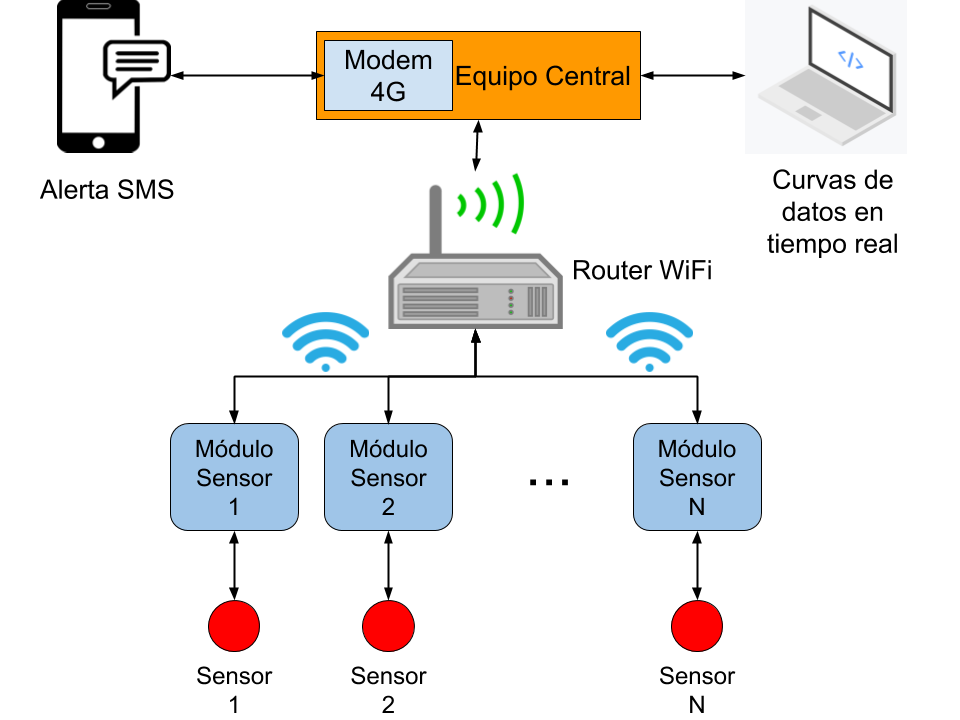
\includegraphics[width=.7\textwidth]{./Figuras/DiagBloques1.png}
\caption{Diagrama en bloques del sistema}
\label{fig:diagBloques}
\end{figure}

\vspace{25px}

El sistema a desarrollar permitirá a los usuarios tener un mayor control y trazabilidad sobre la cadena de frío de sus productos sin tener que dedicar recursos humanos extra para dicha tarea.\newline
El envío de alertas por SMS hace posible a los usuarios conocer el funcionamiento de los equipos de refrigeración en cualquier lugar donde cuenten con cobertura celular.\newline
Finalmente, como puede verse en la Figura 1, el hecho de utilizar una red WiFi provee de gran flexibilidad al sistema de monitoreo, ya que el equipo central y los sensores pueden estar muy distantes o incluso en distintas habitaciones.\newline 


\section{Identificación y análisis de los interesados}
\label{sec:interesados}


\begin{table}[ht]
%\caption{Identificación de los interesados}
%\label{tab:interesados}
\begin{tabularx}{\linewidth}{@{}|l|X|X|l|@{}}
\hline
\rowcolor[HTML]{C0C0C0} 
Rol           & Nombre y Apellido & Organización 	& Puesto 	\\ \hline
Cliente       & \clientename      &\empclientename	& Co Fundador\\ \hline
Responsable   & \authorname       & FIUBA        	& Alumno 	\\ \hline
Orientador    & \supname	      & \pertesupname 	& Director	Trabajo final \\ \hline
Usuario final & Empresa Farmacéutica &  -            	&    -    	\\ \hline
\end{tabularx}
\end{table}

 
\begin{itemize}
\item Cliente: \clientename, tiene una visión muy clara de las características más importantes que debe tener el producto y de la necesidad que debe satisfacer. 
\item Orientador: \supname, tiene una amplia trayectoria en el desarrollo de sistemas electrónicos y gestión de proyectos. Es por ello que va a poder brindarme soporte tanto en el diseño e implementación del Hardware y Firmware, como en la planificación del proyecto.
\end{itemize}




\section{1. Propósito del proyecto}
\label{sec:proposito}

El propósito de este proyecto es realizar un sistema de monitoreo y trazabilidad de temperatura que pueda utilizarse principalmente para asegurar la integridad de los medicamentos que requieran cadena de frío, utilizando para ello una red con tecnología WiFi que otorgue mayor flexibilidad para poder adaptar el sistema a las distintas necesidades de los clientes, y un módem celular para poder enviar alertas por SMS.


\section{2. Alcance del proyecto}
\label{sec:alcance}

El desarrollo del proyecto propuesto incluye:
\begin{itemize}
    \item I+D del Hardware:
        \begin{itemize}
            \item Equipo sensor
            \item Equipo central
        \end{itemize}
    \item Desarrollo del Firmware para:
        \begin{itemize}
            \item Equipo sensor
            \item Equipo central
        \end{itemize}
    \item Implementación de un prototipo funcional formado por:
        \begin{itemize}
            \item 2 (dos) equipos sensores
            \item 1 (uno) equipo central
        \end{itemize}

El desarrollo del proyecto NO incluye la puesta en marcha de un sistema de monitoreo completo con equipos de refrigeración en un centro de almacenaje de medicamentos real.
\end{itemize}




\section{3. Supuestos del proyecto}
\label{sec:supuestos}

Para el desarrollo del presente proyecto se supone que:

\begin{itemize}
\item Se podrá disponer de todos los materiales necesarios para el desarrollo de los prototipos, tales como PCB y componentes electrónicos diversos.
\item Se adquirirán los conocimientos necesarios a lo largo del cursado de la carrera de Especialización en Sistemas Embebidos.
\item Se podrá disponer de todas las herramientas de software necesarias para el diseño de PCB.
\item Se podrá disponer de todas las herramientas de software necesarias para la implementación del Firmware, tales como compiladores y debuggers.
\end{itemize}


\section{4. Requerimientos}
\label{sec:requerimientos}

\begin{enumerate}
\item Requerimientos del Sistema
	\begin{enumerate}
	\item Las mediciones de temperatura deben ser en grados Celcius.
	\item Las mediciones de temperatura deben realizarse en intervalos regulares.
	\item El usuario debe poder configurar a través de una interfaz gráfica los siguientes parámetros: rango de temperatura de cada sensor, numero de teléfono de los usuarios para enviar alerta por SMS, período de medición de temperatura.
    \item El equipo central debe poder almacenar un histórico de mediciones de por lo menos las ultimas 2 semanas de funcionamiento.
	\item El equipo central debe poder enviar SMS de alerta a por lo menos 10 usuarios.
	\end{enumerate}
\item Requerimientos de Hardware
	\begin{enumerate}
	\item Tanto el equipo central como los nodos sensores deben contar con batería de respaldo para poder seguir funcionando ante un corte de energía.
	\item Tanto el equipo central como los nodos sensores deben poder conectarse mediante WiFi.
	\end{enumerate}
\item Requerimientos de Firmware
	\begin{enumerate}
	\item El firmware de todos los equipos deberá ser escrito en lenguajes C y C++.
	\item Se utilizará lenguaje Python para desarrollar herramientas que permitan automatizar procesos repetitivos.
    \item Se desarrollarán tests para probar el correcto funcionamiento del firmware.
	\end{enumerate}
\item Requerimientos de trabajo
	\begin{enumerate}
	\item Se utilizará git para el control de versiones.
	\item Se utilizará github para almacenar los repositorios remotos.
    \item Se utilizará el gestor de proyectos de github para administrar los issues del proyecto.
	\end{enumerate}
\end{enumerate}



\section{Historias de usuarios (\textit{Product backlog})}
\label{sec:backlog}

\begin{enumerate}
    \item Un usuario debe poder acceder a cada sensor para conocer la temperatura actual de cada heladera. (3 story points).
    \item Un usuario debe poder acceder al equipo central para ver un histórico de temperaturas de las heladeras. (5 story points).
    \item Un usuario debe poder recibir alertas por SMS para saber que una temperatura esta fuera de rango. (8 story points).
    \item Un usuario debe poder recibir alertas por SMS para saber que se produjo un corte de energía en una heladera. (8 story points).
    \item Un usuario debe poder enviar un SMS al equipo para detener una alerta de SMS. (5 story points).
    \item Un técnico instalador debe poder acceder a la agenda de contactos para dar de alta un nuevo usuario. (5 story points).
    \item Un técnico instalador debe poder dar de alta un nuevo sensor para medir temperatura en una heladera. (13 story points).
\end{enumerate}

\section{5. Entregables principales del proyecto}
\label{sec:entregables}

\begin{itemize}
\item Circuito esquemático
\item Prototipo funcional
\item Código fuente
\item Manual de usuario
\item Informe final

\end{itemize}



\section{6. Desglose del trabajo en tareas}
\label{sec:wbs}

\begin{enumerate}
\item Organización del proyecto (45hs).
	\begin{enumerate}
	\item Búsqueda, instalación y configuración de herramientas para gestión (5hs).
	\item Elaboración del informe de planificación del proyecto (40hs).
	\end{enumerate}
\item I+D Hardware (216hs).
	\begin{enumerate}
	\item Investigación y selección de módulos WiFi (8hs).
	\item Investigación y selección del modem 4G (8hs).
	\item Investigación y selección del sensor de temperatura (8hs).
	\item Investigación y selección del microcontrolador para el nodo sensor (8hs).
	\item Investigación y selección del microcontrolador para el equipo central (8hs).
	\item Investigación y selección de la batería y monitor de carga para equipo central y nodo sensor (16hs).
	\item Desarrollo del circuito esquemático del modulo sensor (40hs).
	\item Desarrollo del circuito esquemático del equipo central (40hs).
	\item Desarrollo del PCB del modulo sensor (40hs).
	\item Desarrollo del PCB del equipo central (40hs).
	\end{enumerate}
\item I+D Firmware (310hs).
	\begin{enumerate}
	\item Investigación de RTOS (16hs).
	\item Instalación y configuración de las herramientas de desarrollo de Firmware (8hs).
	\item Configuración de los repositorios de Firmware (8hs).
	\item Diseño de la arquitectura de Software (30hs).
	\item Desarrollo de las tareas para comunicación WiFi (40hs).
	\item Desarrollo de las tareas para comunicación con módem celular (80hs).
	\item Desarrollo de las tareas para lectura de sensor de temperatura (8hs).
	\item Desarrollo de las tareas para administración del sistema (80hs).
	\item Integración de todas las tareas (40hs).
	\end{enumerate}
\item Montaje y testeo del Hardware (50hs).
	\begin{enumerate}
	\item Montaje de la placa del nodo sensor (8hs).
	\item Montaje de la placa del equipo central (8hs).
	\item Programación base del nodo sensor (1hs).
	\item Programación base del equipo central (1hs).
	\end{enumerate}
\item Testeo del Firmware (64hs).
	\begin{enumerate}
	\item Testing de la comunicación WiFi (8hs).
	\item Testing del envío de SMS (8hs).
	\item Testing de la configuración del equipo central (8hs).
	\item Testing de la lectura del sensor (4hs).
	\item Testing del sistema completo (40hs).
	\end{enumerate}
\item Defensa del Proyecto Final (68hs).
	\begin{enumerate}
	\item Elaboración del informe final (50hs).
	\item Elaboración de la presentación final (18hs).
	\end{enumerate}
\end{enumerate}

Cantidad total de horas: 715 hs.

\section{7. Diagrama de Activity On Node}
\label{sec:AoN}

\usetikzlibrary{positioning}

%circles
\tikzstyle{startstop} = [draw=black, circle, text centered, text width=1cm, fill=white!30, rounded corners=.7ex]
\tikzstyle{break}     = [draw=black, circle, text centered, text width=0.5cm, fill=white!30]

%tasks
\tikzstyle{tasktype1} = [draw=black,rectangle, text centered, text width=2cm, fill=gray!30]
\tikzstyle{tasktype2} = [draw=black,rectangle, text centered, text width=2cm, fill=red!30]
\tikzstyle{tasktype3} = [draw=black,rectangle, text centered, text width=2cm, fill=green!30]
\tikzstyle{tasktype4} = [draw=black,rectangle, text centered, text width=2cm, fill=blue!30]
\tikzstyle{tasktype5} = [draw=black,rectangle, text centered, text width=2cm, fill=orange!30]
\tikzstyle{tasktype6} = [draw=black,rectangle, text centered, text width=2cm, fill=yellow!50]

%Esto  es para habilitar el uso de > para las arrows, si no se agrega aparece un error de compilacion
\shorthandoff{>}
\tikzstyle{arrow} = [thick,->,>=stealth]

\begin{tikzpicture}[node distance=1cm]
    \node (start) [startstop] {\tiny INICIO\\23/10/20};
    %Section 1 tasks
    \node (task1-1) [tasktype1, right of=start, xshift=1.5cm    ]   {\tiny 1.1 Herramientas para gestión \\t = 5};
    \node (task1-2) [tasktype1, right of=task1-1, xshift=2cm  ]   {\tiny 1.2 Informe del proyecto \\t = 40};
    %Section 2 tasks
    \node (task2-1) [tasktype2, right of=task1-2, xshift=2cm, yshift= 1cm ] {\tiny 2.1 Selección de módulo WiFi \\t = 8};
    \node (task2-2) [tasktype2, right of=task1-2, xshift=2cm, yshift=-1cm ] {\tiny 2.2 Selección de modem 4G \\t = 8};
    \node (task2-3) [tasktype2, right of=task2-1, xshift=2cm ] {\tiny 2.3 Selección de sensor de temperatura \\t =  8};
    \node (task2-4) [tasktype2, right of=task2-3, xshift=2cm ] {\tiny 2.4 Selección de microcontrolador del nodo sensor \\t = 8};
    \node (task2-5) [tasktype2, right of=task2-2, xshift=2cm ] {\tiny 2.5 Selección de microcontrolador del equipo central \\t = 8};
    \node (task2-6) [tasktype2, below of=task1-1, yshift=-3cm ]{\tiny 2.6 Selección de batería y monitor de carga \\t = 16};
    \node (task2-7) [tasktype2, right of=task2-6, xshift=2cm, yshift= 1cm ]  {\tiny 2.7 Circuito esquemático del modulo sensor \\t = 40};
    \node (task2-8) [tasktype2, below of=task2-7, yshift=-1cm] {\tiny 2.8 Circuito esquemático del equipo central \\t = 40};
    \node (task2-9) [tasktype2, right of=task2-7, xshift=2cm ] {\tiny 2.9 PCB del modulo sensor \\t =  40};
    \node (task2-10)[tasktype2, right of=task2-8, xshift=2cm ] {\tiny 2.10 PCB del equipo central \\t =  40};

    %section 3 tasks
    \node (task3-1) [tasktype3, below of=task2-6, yshift=-5cm ]{\tiny 3.1 Investigación de RTOS \\t = 16};
    \node (task3-2) [tasktype3, right of=task3-1, xshift=2cm ] {\tiny 3.2 Instalación y configuración de las herramientas de desarrollo de Firmware \\t = 8};
    \node (task3-3) [tasktype3, right of=task3-2, xshift=2cm, yshift=1cm ] {\tiny 3.3 Configuración de los repositorios de Firmware \\t = 8};
    \node (task3-4) [tasktype3, below of=task3-3, yshift=-1cm ]{\tiny 3.4 Diseño de la arquitectura de Software \\t = 30};
    \node (task3-5) [tasktype3, right of=task3-3, xshift=2cm, yshift=2cm ] {\tiny 3.5 Desarrollo de tareas para comunicación WiFi \\t = 40};
    \node (task3-6) [tasktype3, below of=task3-5, yshift=-1cm ] {\tiny 3.6 Desarrollo de tareas para comunicación con módem celular \\t = 80};
    \node (task3-7) [tasktype3, below of=task3-6, yshift=-1cm ] {\tiny 3.7 Desarrollo de tareas para lectura de sensor de temperatura \\t = 8};
    \node (task3-8) [tasktype3, below of=task3-7, yshift=-1cm ] {\tiny 3.8 Desarrollo de tareas para administración del sistema \\t = 80};
    \node (task3-9) [tasktype3, below of=task3-1, yshift=-4.5cm ] {\tiny 3.9 Integración de todas las tareas \\t = 40};

    %section 4 tasks
    \node (task4-1) [tasktype4, right of=task2-9, xshift=2cm ] {\tiny 4.1 Montaje de la placa del nodo sensor \\t = 8};
    \node (task4-2) [tasktype4, right of=task2-10, xshift=2cm ] {\tiny 4.2 Montaje de la placa del equipo central \\t = 8};
    \node (task4-3) [tasktype4, right of=task4-1, xshift=2cm ] {\tiny 4.3 Programación base del nodo sensor \\t = 1};
    \node (task4-4) [tasktype4, right of=task4-2, xshift=2cm ] {\tiny 4.4 Programación base del equipo central \\t = 1};

    %section 5 tasks
    \node (task5-1) [tasktype5, right of=task3-5, xshift=2cm ] {\tiny 5.1 Testing de la comunicación WiFi \\t = 8};
    \node (task5-2) [tasktype5, right of=task3-6, xshift=2cm ] {\tiny 5.2 Testing del envío de SMS \\t = 8};
    \node (task5-3) [tasktype5, right of=task3-8, xshift=2cm ] {\tiny 5.3 Testing de la configuración del equipo central \\t = 8};
    \node (task5-4) [tasktype5, right of=task3-7, xshift=2cm ] {\tiny 5.4 Testing del sensor \\t = 4};
    \node (task5-5) [tasktype5, right of=task3-9, xshift=2cm ] {\tiny 5.5 Testing del sistema completo \\t = 40};

    %section 6 tasks
    \node (task6-1) [tasktype6, right of=task5-5, xshift=2cm ] {\tiny 6.1 Elaboración del informe final \\t = 50};
    \node (task6-2) [tasktype6, right of=task6-1, xshift=2cm ] {\tiny 6.2 Elaboración de la presentación final \\t = 18};

    %end
    \node (end) [startstop, right of=task6-2, xshift=2cm ] {\tiny FIN};

    %lines and arrows
    \draw[arrow] (start) -- (task1-1);
    \draw[arrow] (task1-1) -- (task1-2);
    \draw[arrow] (task1-2) -- node {} ++(1.5cm,0) -- node {} ++(0, 1cm) -- (task2-1);
    \draw[arrow] (task1-2) -- node {} ++(1.5cm,0) -- node {} ++(0,-1cm) -- (task2-2);
    \draw[arrow] (task2-1) -- (task2-3);
    \draw[arrow] (task2-3) -- (task2-4);
    \draw[arrow] (task2-2) -- (task2-5);
    \draw[arrow] (task2-4) -- node {} ++(1.5cm,0) -- node {} ++(0,-3.1cm) -- node {} ++(-16.7cm,0) -- node {} ++(0,-1.9cm) -- (task2-6);
    \draw[arrow] (task2-5) -- node {} ++(4.5cm,0) -- node {} ++(0,-1.1cm) -- node {} ++(-16.7cm,0) -- node {} ++(0,-7.9cm) -- (task3-1);
    \draw[arrow] (task2-6) -- node {} ++(1.5cm,0) -- node {} ++(0, 1cm) -- (task2-7);
    \draw[arrow] (task2-6) -- node {} ++(1.5cm,0) -- node {} ++(0,-1cm) -- (task2-8);
    \draw[arrow] (task2-7) -- (task2-9);
    \draw[arrow] (task2-8) -- (task2-10);
    \draw[arrow] (task3-1) -- (task3-2);
    \draw[arrow] (task3-2) -- node {} ++(1.5cm,0) -- node {} ++(0, 1cm) -- (task3-3);
    \draw[arrow] (task3-2) -- node {} ++(1.5cm,0) -- node {} ++(0,-1cm) -- (task3-4);
    \draw[arrow] (task2-9) -- (task4-1);
    \draw[arrow] (task2-10) -- (task4-2);
    \draw[arrow] (task4-1) -- (task4-3);
    \draw[arrow] (task4-2) -- (task4-4);

    \draw[arrow] (task3-3) -- node {} ++(1.3cm,0) -- node {} ++(0,-1cm) -- node {} ++(0.3cm,0) -- node {} ++(0,-3cm) --     (task3-8);
    \draw[arrow] (task3-4) -- node {} ++(1.3cm,0) -- node {} ++(0, 1cm) -- node {} ++(0.3cm,0) -- node {} ++(0, 3cm) --     (task3-5);
    \draw[arrow] (task3-3) -- node {} ++(1.3cm,0) -- node {} ++(0,-1cm) -- node {} ++(0.3cm,0) -- node {} ++(0,-1cm) --   (task3-7);
    \draw[arrow] (task3-4) -- node {} ++(1.3cm,0) -- node {} ++(0, 1cm) -- node {} ++(0.3cm,0) -- node {} ++(0, 1cm) --   (task3-6);

    \draw[arrow] (task3-5) -- (task5-1);
    \draw[arrow] (task3-6) -- (task5-2);
    \draw[arrow] (task3-7) -- (task5-4);
    \draw[arrow] (task3-8) -- (task5-3);

    \draw[arrow] (task4-3) -- node {} ++(1.5cm,0) -- node {} ++(0,-11.1cm)  -- node {} ++(-16.7cm,0) -- node {} ++(0,-1.4cm) -- (task3-9);
    \draw[arrow] (task4-4) -- node {} ++(1.5cm,0) -- node {} ++(0,-9.1cm)   -- node {} ++(-16.7cm,0) -- node {} ++(0,-1.4cm) -- (task3-9);
    \draw[arrow] (task5-1) -- node {} ++(1.5cm,0) -- node {} ++(0,-7.1cm)   -- node {} ++(-16.7cm,0) -- node {} ++(0,-1.4cm) -- (task3-9);
    \draw[arrow] (task5-2) -- node {} ++(1.5cm,0) -- node {} ++(0,-5.1cm)   -- node {} ++(-16.7cm,0) -- node {} ++(0,-1.4cm) -- (task3-9);
    \draw[arrow] (task5-4) -- node {} ++(1.5cm,0) -- node {} ++(0,-3.1cm)   -- node {} ++(-16.7cm,0) -- node {} ++(0,-1.4cm) -- (task3-9);
    \draw[arrow] (task5-3) -- node {} ++(1.5cm,0) -- node {} ++(0,-1.1cm)   -- node {} ++(-16.7cm,0) -- node {} ++(0,-1.4cm) -- (task3-9);
    
    \draw[arrow] (task3-9) -- (task5-5);
    \draw[arrow] (task5-5) -- (task6-1);
    \draw[arrow] (task6-1) -- (task6-2);
    \draw[arrow] (task6-2) -- (end);

\end{tikzpicture}\vspace{2cm}                                     

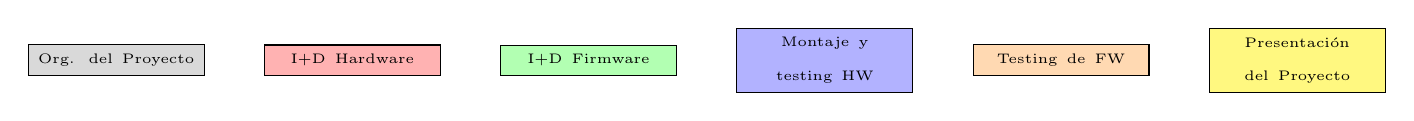
\begin{tikzpicture}

%tasks
\tikzstyle{tasktype1} = [draw=black,rectangle, text centered, text width=2cm, fill=gray!30]
\tikzstyle{tasktype2} = [draw=black,rectangle, text centered, text width=2cm, fill=red!30]
\tikzstyle{tasktype3} = [draw=black,rectangle, text centered, text width=2cm, fill=green!30]
\tikzstyle{tasktype4} = [draw=black,rectangle, text centered, text width=2cm, fill=blue!30]
\tikzstyle{tasktype5} = [draw=black,rectangle, text centered, text width=2cm, fill=orange!30]
\tikzstyle{tasktype6} = [draw=black,rectangle, text centered, text width=2cm, fill=yellow!50]

\node (task1) [tasktype1  ]                             {\tiny Org. del Proyecto};
\node (task2) [tasktype2, right of=task1, xshift=2cm ]  {\tiny I+D Hardware};
\node (task3) [tasktype3, right of=task2, xshift=2cm ]  {\tiny I+D Firmware};
\node (task4) [tasktype4, right of=task3, xshift=2cm ]  {\tiny Montaje y testing HW};
\node (task5) [tasktype5, right of=task4, xshift=2cm ]  {\tiny Testing de FW};
\node (task6) [tasktype6, right of=task5, xshift=2cm ]  {\tiny Presentación del Proyecto};

\end{tikzpicture}                                     




\section{8. Diagrama de Gantt}
\label{sec:gantt}

\begin{consigna}{red}
Utilizar el software Gantter for Google Drive o alguno similar para dibujar el diagrama de Gantt.

Existen muchos programas y recursos \textit{online} para hacer diagramas de gantt, entre las cuales destacamos:

\begin{itemize}
\item Planner
\item GanttProject
\item Trello + \textit{plugins}. En el siguiente link hay un tutorial oficial: \\ \url{https://blog.trello.com/es/diagrama-de-gantt-de-un-proyecto}
\item Creately, herramienta online colaborativa. \\\url{https://creately.com/diagram/example/ieb3p3ml/LaTeX}
\item Se puede hacer en latex con el paquete \textit{pgfgantt}\\ \url{http://ctan.dcc.uchile.cl/graphics/pgf/contrib/pgfgantt/pgfgantt.pdf}
\end{itemize}

Pegar acá una captura de pantalla del diagrama de Gantt, cuidando que la letra sea suficientemente grande como para ser legible. 
Si el diagrama queda demasiado ancho, se puede pegar primero la ``tabla'' del Gantt y luego pegar la parte del diagrama de barras del diagrama de Gantt.

Configurar el software para que en la parte de la tabla muestre los códigos del EDT (WBS).\\
Configurar el software para que al lado de cada barra muestre el nombre de cada tarea.\\
Revisar que la fecha de finalización coincida con lo indicado en el Acta Constitutiva.

En la figura \ref{fig:gantt}, se muestra un ejemplo de diagrama de gantt realizado con el paquete de \textit{pgfgantt}. En la plantilla pueden ver el código que lo genera y usarlo de base para construir el propio.

\begin{figure}[htbp]
\begin{center}
\begin{ganttchart}{1}{12}
  \gantttitle{2020}{12} \\
  \gantttitlelist{1,...,12}{1} \\
  \ganttgroup{Group 1}{1}{7} \\
  \ganttbar{Task 1}{1}{2} \\
  \ganttlinkedbar{Task 2}{3}{7} \ganttnewline
  \ganttmilestone{Milestone o hito}{7} \ganttnewline
  \ganttbar{Final Task}{8}{12}
  \ganttlink{elem2}{elem3}
  \ganttlink{elem3}{elem4}
\end{ganttchart}
\end{center}
\caption{Diagrama de gantt de ejemplo}
\label{fig:gantt}
\end{figure}

\end{consigna}

\section{9. Matriz de uso de recursos de materiales}
\label{sec:recursos}


\begin{table}
\label{tab:recursos}
\centering
\begin{tabularx}{\linewidth}{@{}|c|X|X|X|X|c|@{}}
\hline
\cellcolor[HTML]{C0C0C0} & \cellcolor[HTML]{C0C0C0} & \multicolumn{4}{c|}{\cellcolor[HTML]{C0C0C0}Recursos requeridos (horas)} \\ \cline{3-6} 
\multirow{-2}{*}{\cellcolor[HTML]{C0C0C0}\begin{tabular}[c]{@{}c@{}}Código\\ WBS\end{tabular}} & \multirow{-2}{*}{\cellcolor[HTML]{C0C0C0}\begin{tabular}[c]{@{}c@{}}Nombre \\ tarea\end{tabular}} & Material 1 & Material 2 & Material 3 & Material 4 \\ \hline
 &  &  &  &  &  \\ \hline
 &  &  &  &  &  \\ \hline
 &  &  &  &  &  \\ \hline
 &  &  &  &  &  \\ \hline
 &  &  &  &  &  \\ \hline
 &  &  &  &  &  \\ \hline
 &  &  &  &  &  \\ \hline
 &  &  &  &  &  \\ \hline 
 &  &  &  &  &  \\ \hline
 &  &  &  &  &  \\ \hline
 &  &  &  &  &  \\ \hline
 &  &  &  &  &  \\ \hline
 &  &  &  &  &  \\ \hline
 &  &  &  &  &  \\ \hline
 &  &  &  &  &  \\ \hline
 &  &  &  &  &  \\ \hline
 &  &  &  &  &  \\ \hline
 &  &  &  &  &  \\ \hline
 &  &  &  &  &  \\ \hline
 &  &  &  &  &  \\ \hline
 &  &  &  &  &  \\ \hline
 &  &  &  &  &  \\ \hline
 &  &  &  &  &  \\ \hline
 &  &  &  &  &  \\ \hline 
 &  &  &  &  &  \\ \hline
 &  &  &  &  &  \\ \hline
 &  &  &  &  &  \\ \hline
 &  &  &  &  &  \\ \hline

\end{tabularx}%
\end{table}


\section{10. Presupuesto detallado del proyecto}
\label{sec:presupuesto}

\begin{consigna}{red}
Si el proyecto es complejo entonces separarlo en partes:
\begin{itemize}
\item Un total global, indicando el subtotal acumulado por cada una de las áreas.
\item El desglose detallado del subtotal de cada una de las áreas.
\end{itemize}

IMPORTANTE: No olvidarse de considerar los COSTOS INDIRECTOS.

\end{consigna}

\begin{table}[htpb]
\centering
\begin{tabularx}{\linewidth}{@{}|X|c|r|r|@{}}
\hline
\rowcolor[HTML]{C0C0C0} 
\multicolumn{4}{|c|}{\cellcolor[HTML]{C0C0C0}COSTOS DIRECTOS} \\ \hline
\rowcolor[HTML]{C0C0C0} 
Descripción &
  \multicolumn{1}{c|}{\cellcolor[HTML]{C0C0C0}Cantidad} &
  \multicolumn{1}{c|}{\cellcolor[HTML]{C0C0C0}Valor unitario} &
  \multicolumn{1}{c|}{\cellcolor[HTML]{C0C0C0}Valor total} \\ \hline
 &
  \multicolumn{1}{c|}{} &
  \multicolumn{1}{c|}{} &
  \multicolumn{1}{c|}{} \\ \hline
 &
  \multicolumn{1}{c|}{} &
  \multicolumn{1}{c|}{} &
  \multicolumn{1}{c|}{} \\ \hline
\multicolumn{1}{|l|}{} &
   &
   &
   \\ \hline
\multicolumn{1}{|l|}{} &
   &
   &
   \\ \hline
\multicolumn{3}{|c|}{SUBTOTAL} &
  \multicolumn{1}{c|}{} \\ \hline
\rowcolor[HTML]{C0C0C0} 
\multicolumn{4}{|c|}{\cellcolor[HTML]{C0C0C0}COSTOS INDIRECTOS} \\ \hline
\rowcolor[HTML]{C0C0C0} 
Descripción &
  \multicolumn{1}{c|}{\cellcolor[HTML]{C0C0C0}Cantidad} &
  \multicolumn{1}{c|}{\cellcolor[HTML]{C0C0C0}Valor unitario} &
  \multicolumn{1}{c|}{\cellcolor[HTML]{C0C0C0}Valor total} \\ \hline
\multicolumn{1}{|l|}{} &
   &
   &
   \\ \hline
\multicolumn{1}{|l|}{} &
   &
   &
   \\ \hline
\multicolumn{1}{|l|}{} &
   &
   &
   \\ \hline
\multicolumn{3}{|c|}{SUBTOTAL} &
  \multicolumn{1}{c|}{} \\ \hline
\rowcolor[HTML]{C0C0C0}
\multicolumn{3}{|c|}{TOTAL} &
   \\ \hline
\end{tabularx}%
\end{table}


\section{11. Matriz de asignación de responsabilidades}
\label{sec:responsabilidades}
\begin{consigna}{red}
Establecer la matriz de asignación de responsabilidades y el manejo de la autoridad completando la siguiente tabla:

\begin{table}[htpb]
\centering
\resizebox{\textwidth}{!}{%
\begin{tabular}{|c|c|c|c|c|c|}
\hline
\rowcolor[HTML]{C0C0C0} 
\cellcolor[HTML]{C0C0C0} &
  \cellcolor[HTML]{C0C0C0} &
  \multicolumn{4}{c|}{\cellcolor[HTML]{C0C0C0}Listar todos los nombres y roles del proyecto} \\ \cline{3-6} 
\rowcolor[HTML]{C0C0C0} 
\cellcolor[HTML]{C0C0C0} &
  \cellcolor[HTML]{C0C0C0} &
  Responsable &
  Orientador &
  Equipo &
  Cliente \\ \cline{3-6} 
\rowcolor[HTML]{C0C0C0} 
\multirow{-3}{*}{\cellcolor[HTML]{C0C0C0}\begin{tabular}[c]{@{}c@{}}Código\\ WBS\end{tabular}} &
  \multirow{-3}{*}{\cellcolor[HTML]{C0C0C0}Nombre de la tarea} &
  \authorname &
  \supname &
  Nombre de alguien &
  \clientename \\ \hline
 &  &  &  &  &  \\ \hline
 &  &  &  &  &  \\ \hline
 &  &  &  &  &  \\ \hline
\end{tabular}%
}
\end{table}

{\footnotesize
Referencias:
\begin{itemize}
	\item P = Responsabilidad Primaria
	\item S = Responsabilidad Secundaria
	\item A = Aprobación
	\item I = Informado
	\item C = Consultado
\end{itemize}
} %footnotesize

Una de las columnas debe ser para el Director, ya que se supone que participará en el proyecto.
A su vez se debe cuidar que no queden muchas tareas seguidas sin ``A'' o ``I''.

Importante: es redundante poner ``I/A'' o ``I/C'', porque para aprobarlo o responder consultas primero la persona debe ser informada.

\end{consigna}

\section{12. Gestión de riesgos}
\label{sec:riesgos}

\begin{consigna}{red}
a) Identificación de los riesgos (al menos cinco) y estimación de sus consecuencias:
 
Riesgo 1: detallar el riesgo (riesgo es algo que si ocurre altera los planes previstos)
\begin{itemize}
\item Severidad (S): mientras más severo, más alto es el número (usar números del 1 al 10).\\
Justificar el motivo por el cual se asigna determinado número de severidad (S).
\item Probabilidad de ocurrencia (O): mientras más probable, más alto es el número (usar del 1 al 10).\\
Justificar el motivo por el cual se asigna determinado número de (O). 
\end{itemize}   

Riesgo 2:
\begin{itemize}
\item Severidad (S): 
\item Ocurrencia (O):
\end{itemize}

Riesgo 3:
\begin{itemize}
\item Severidad (S): 
\item Ocurrencia (O):
\end{itemize}


b) Tabla de gestión de riesgos:      (El RPN se calcula como RPN=SxO)

\begin{table}[htpb]
\centering
\begin{tabularx}{\linewidth}{@{}|X|c|c|c|c|c|c|@{}}
\hline
\rowcolor[HTML]{C0C0C0} 
Riesgo & S & O & RPN & S* & O* & RPN* \\ \hline
       &   &   &     &    &    &      \\ \hline
       &   &   &     &    &    &      \\ \hline
       &   &   &     &    &    &      \\ \hline
       &   &   &     &    &    &      \\ \hline
       &   &   &     &    &    &      \\ \hline
\end{tabularx}%
\end{table}

Criterio adoptado: 
Se tomarán medidas de mitigación en los riesgos cuyos números de RPN sean mayores a...

Nota: los valores marcados con (*) en la tabla corresponden luego de haber aplicado la mitigación.

c) Plan de mitigación de los riesgos que originalmente excedían el RPN máximo establecido:
 
Riesgo 1: plan de mitigación (si por el RPN fuera necesario elaborar un plan de mitigación).
  Nueva asignación de S y O, con su respectiva justificación:
  - Severidad (S): mientras más severo, más alto es el número (usar números del 1 al 10).
          Justificar el motivo por el cual se asigna determinado número de severidad (S).
  - Probabilidad de ocurrencia (O): mientras más probable, más alto es el número (usar del 1 al 10).
          Justificar el motivo por el cual se asigna determinado número de (O).

Riesgo 2: plan de mitigación (si por el RPN fuera necesario elaborar un plan de mitigación).
 
Riesgo 3: plan de mitigación (si por el RPN fuera necesario elaborar un plan de mitigación).

\end{consigna}


\section{13. Gestión de la calidad}
\label{sec:calidad}

\begin{consigna}{red}
Para cada uno de los requerimientos del proyecto indique:
\begin{itemize} 
\item Req \#1: copiar acá el requerimiento.

Verificación y validación:

\begin{itemize}
\item Verificación para confirmar si se cumplió con lo requerido antes de mostrar el sistema al cliente. Detallar 
\item Validación con el cliente para confirmar que está de acuerdo en que se cumplió con lo requerido. Detallar  
\end{itemize}

\end{itemize}

Tener en cuenta que en este contexto se pueden mencionar simulaciones, cálculos, revisión de hojas de datos, consulta con expertos, mediciones, etc.

\end{consigna}

\section{14. Comunicación del proyecto}
\label{sec:comunicaciones}

El plan de comunicación del proyecto es el siguiente:

\begin{table}[htpb]
\centering
\begin{tabularx}{\linewidth}{@{}|X|C{2.4cm}|C{3cm}|C{1.8cm}|C{2cm}|C{2.1cm}|@{}}
\hline
\rowcolor[HTML]{C0C0C0} 
\multicolumn{6}{|c|}{\cellcolor[HTML]{C0C0C0}PLAN DE COMUNICACIÓN DEL PROYECTO}           \\ \hline
\rowcolor[HTML]{C0C0C0} 
¿Qué comunicar? & Audiencia & Propósito & Frecuencia & Método de comunicac. & Responsable \\ \hline
                &           &           &            &                      &             \\ \hline
                &           &           &            &                      &             \\ \hline
                &           &           &            &                      &             \\ \hline
                &           &           &            &                      &             \\ \hline
                &           &           &            &                      &             \\ \hline
\end{tabularx}
\end{table}

\section{15. Gestión de compras}
\label{sec:compras}

\begin{consigna}{red}
En caso de tener que comprar elementos o contratar servicios:
a) Explique con qué criterios elegiría a un proveedor.
b) Redacte el Statement of Work correspondiente.
\end{consigna}

\section{16. Seguimiento y control}
\label{sec:seguimiento}

\begin{consigna}{red}
Para cada tarea del proyecto establecer la frecuencia y los indicadores con los se seguirá su avance y quién será el responsable de hacer dicho seguimiento y a quién debe comunicarse la situación (en concordancia con el Plan de Comunicación del proyecto).

El indicador de avance tiene que ser algo medible, mejor incluso si se puede medir en \% de avance. Por ejemplo,se pueden indicar en esta columna cosas como ``cantidad de conexiones ruteadeas'' o ``cantidad de funciones implementadas'', pero no algo genérico y ambiguo como ``\%'', porque el lector no sabe porcentaje de qué cosa.

\end{consigna}

\begin{longtable}{|m{1cm}|m{3.5cm}|m{2.2cm}|m{2cm}|m{3cm}|m{1.5cm}|}
\hline
\rowcolor[HTML]{C0C0C0} 
\multicolumn{6}{|c|}{\cellcolor[HTML]{C0C0C0}SEGUIMIENTO DE AVANCE}                                                                       \\ \hline
\rowcolor[HTML]{C0C0C0} 
Tarea del WBS 			& Indicador de avance & Frecuencia de reporte & Resp. de seguimiento & Persona a ser informada & Método de comunic. \\ \hline
\endfirsthead

\hline
\rowcolor[HTML]{C0C0C0} 
\multicolumn{6}{c}{\cellcolor[HTML]{C0C0C0}SEGUIMIENTO DE AVANCE}                                                                       \\ \hline
\rowcolor[HTML]{C0C0C0} 
Tarea del WBS 			& Indicador de avance & Frecuencia de reporte & Resp. de seguimiento & Persona a ser informada & Método de comunic. \\ \hline
\endhead

\multicolumn{6}{c}{Continúa}
\endfoot

\endlastfoot

1.1	& Fecha de inicio  & Única vez al comienzo & \authorname & \clientename, \supname & email \\ \hline
2.1	& Avance de las subtareas  & Mensual mientras dure la tarea & \authorname & \clientename, \supname & email \\ \hline

\end{longtable}

\begin{table}[!htpb]
\centering
%\begin{tabularx}{\linewidth}{@{}|X|X|X|X|X|X|@{}}
\begin{tabularx}{\linewidth}{@{}|X|C{2.5cm}|C{3cm}|C{2cm}|C{2cm}|C{2.5cm}|@{}}
\hline
\rowcolor[HTML]{C0C0C0} 
\multicolumn{6}{|c|}{\cellcolor[HTML]{C0C0C0}SEGUIMIENTO DE AVANCE}                                                                       \\ \hline
\rowcolor[HTML]{C0C0C0} 
Tarea del WBS & Indicador de avance & Frecuencia de reporte & Resp. de seguimiento & Persona a ser informada & Método de comunic. \\ \hline
 &  &  &  &  &  \\ \hline
 &  &  &  &  &  \\ \hline
 &  &  &  &  &  \\ \hline
 &  &  &  &  &  \\ \hline
 &  &  &  &  &  \\ \hline
\end{tabularx}%
%}
\end{table}

\section{17. Procesos de cierre}    
\label{sec:cierre}

\begin{consigna}{red}
Establecer las pautas de trabajo para realizar una reunión final de evaluación del proyecto, tal que contemple las siguientes actividades:

\begin{itemize}
\item Pautas de trabajo que se seguirán para analizar si se respetó el Plan de Proyecto original:
 - Indicar quién se ocupará de hacer esto y cuál será el procedimiento a aplicar. 
\item Identificación de las técnicas y procedimientos útiles e inútiles que se utilizaron, y los problemas que surgieron y cómo se solucionaron:
 - Indicar quién se ocupará de hacer esto y cuál será el procedimiento para dejar registro.
\item Indicar quién organizará el acto de agradecimiento a todos los interesados, y en especial al equipo de trabajo y colaboradores:
  - Indicar esto y quién financiará los gastos correspondientes.
\end{itemize}

\end{consigna}


\end{document}
